
\subsection{Backward Difference Formulas}

Backward Difference Formulas (BDF) are popular methods for stiff problems,
and are derived by differentiating a polynomial representation of
$s$ past solutions, $x_{n-i}$ for $i=1,\ldots,s$, and setting the
derivative $\dot{x}(t_{n})=f(t_{n},x_{n})$. For evenly spaced intervals,
$\Delta t=t_{n}-t_{n-1}$, an $s$-step BDF method (BDF$s$) is given
by
\begin{equation}
\dot{x}_{n}=\bar{f}(t_{n},x_{n})=\frac{1}{\Delta t\,\beta_{0}}\sum_{i=0}^{s}\alpha_{i}\, x_{n-i}\label{rythmos:eq:bdf_x_dot}
\end{equation}
where $\alpha_{0}$ is normally scaled to one, and the order is equal
to the number of steps, $s$.

The nonlinear time step equation to advance the solution from $t_{n-1}$
to $t_{n}$ is then formed by substituting $\dot{x}=\dot{x}_{n}$
in (\ref{rythmos:eq:bdf_x_dot}), $x=x_{n}$ and $t=t_{n}$ into (\ref{rythmos:eq:dae})
to obtain 
\begin{equation}
f\left(\left[\frac{1}{\Delta t\,\beta_{0}}\sum_{i=0}^{s}\alpha_{i}\, x_{n-i}\right],x_{n},t_{n}\right)=0.\label{rythmos:eq:bdf_dae_ne}
\end{equation}
One can immediately identify the BDF time step equations (\ref{rythmos:eq:bdf_dae_ne})
with the general form of the time step equations (\ref{rythmos:eq:r})
and with unknown solution variables $z=x_{n}$. All of the other state
variables $x_{n-i}$, for $i=1\ldots s$, are given.

Note that the first-order BDF method with $p=1$, $\alpha_{0}=1$
and $\alpha_{1}=-1$ is simply the standard backward Euler time integration
method \cite{AscherPetzold}.

When considering a general Newton-like method for solving (\ref{rythmos:eq:bdf_dae_ne}),
note that the Newton Jacobian of these equations is 
\begin{equation}
\Jac{r}{z}=\frac{\alpha_{0}}{\Delta t\,\beta_{0}}\Jac{f}{\dot{x}}+\Jac{f}{x},\label{rythmos:eq:W_bdf}
\end{equation}
which is evaluated at the point $\dot{x}$ in (\ref{rythmos:eq:bdf_x_dot}),
$x=x_{n}$ and $t=t_{n}$. One can immediately identify (\ref{rythmos:eq:W_bdf})
with the general form of the matrix $M$ in (\ref{rythmos:eq:W})
where $\alpha=\alpha_{0}/(\Delta t\,\beta_{0})$ and $\beta=1$. Note
that the Jacobian (\ref{rythmos:eq:W_bdf}) is the exact Jacobian
for the nonlinear time step equations; this will not be true for some
of the other methods.

There are three major variations of BDFs for variable time-step methods:
fixed-coefficient formulas, variable-coefficient formulas, and fixed-leading-coefficient
formulas. The fixed-coefficient formulas assume evenly spaced intervals
so that the coefficients are fixed and can be precomputed for all
orders\cite[p. 130]{AscherPetzold}. However when the time-step size
changes the solution must be interpolated to evenly spaced intervals,
and the amount of work for the interpolation is proportional to the
number of equations in the system. Jackson and Sacks-Davis\cite{Jackson1980}
have noted that fixed-coefficient formulas have worse stability properties
than the other two variations. Also there can be an additional computational
savings if $\jac{f}{x}$ is constant and the time step and order are
consistently updated, fewer matrix factorizations and evaluations
are possible.

For variable-coefficient formulas, the coefficients need to be recalculated
if the time step has changed in the past $s$ steps, which the amount
of work depends on the number of steps but is independent of the number
of equations. As noted earlier, variable-coefficient formulas have
better stability properties which allow larger changes in time step
and order during the solution of the problem. This can reduce the
overall computational costs through larger time steps. It should be
noted that the nonlinear matrix will need to be refactorized even
if $\jac{f}{x}$ is constant, when the time step has changed in the
past $s$ steps thus increasing the of variable-coefficient formulas.

Variable-coefficient formulas would be the preferred approach except
for the when $\jac{f}{x}$ is constant, when the time step has changed
in the past $s$ steps. Jackson and Sacks-Davis\cite{Jackson1980}
noted that if the leading coefficient, $\alpha_{0}$, is kept constant
this exception can be removed, and these methods have been termed
fixed-leading-coefficient formulas. thus is a hybrid between the two
methods and tries to obtain the best of both worlds.


\paragraph*{Fixed-Leading-Coefficient Formula\cite{BDF-FLC}}

To begin, we need a predictor polynomial, $\phi_{p}(t)$, that uses
the past solution values (possibility at uneven intervals)
\[
\phi_{p}(t_{n-i})=x_{n-i}\mbox{{\,\,\,\ for\,\,}}i=1,\ldots,s
\]
and the time derivative
\[
\dot{\phi}_{p}(t_{n-i})=\dot{x}_{n-i}
\]
A corrector polynomial, $\phi_{c}(t)$, is constructed on even intervals
of $\Delta t_{n}=t_{n}-t_{n-1}$, and is equal to $\phi_{p}(t)$ at
those locations. 
\begin{eqnarray*}
\phi_{c}(t_{n}) & = & x_{n}\\
\phi_{c}(t_{n}-i\Delta t_{n}) & = & \phi_{p}(t_{n}-i\Delta t_{n})\mbox{{\,\,\,\ for\,\,} }i=1,\ldots,s
\end{eqnarray*}
Thus $\phi_{c}$ passes through the unknown solution at $t_{n}$.
The schematic of these polynomials are shown in Fig.~\ref{rythmos:fig:BDF2-schematic}
for a BDF2 method. Note that in this illustration, the variable time
stepping is increasing, thus $t_{n}-2\Delta t_{n}$ is further back
in time than $t_{n-2}$.

\begin{figure}
\centering{}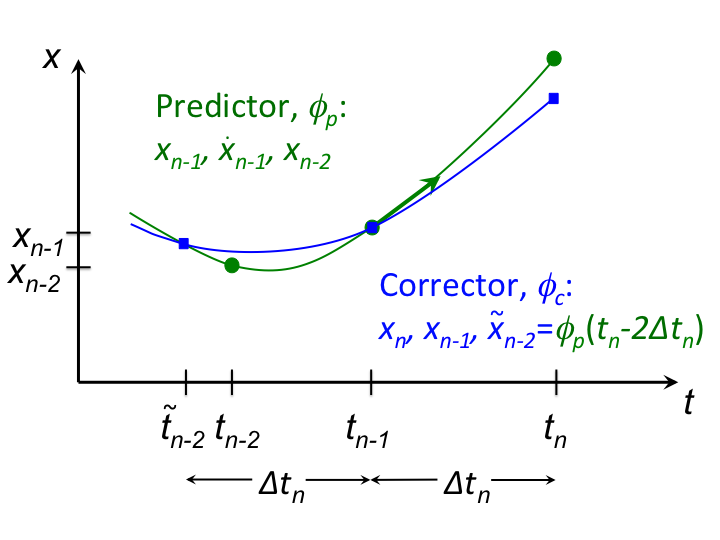
\includegraphics[width=4in]{figures/BDF2}\caption{Schematic of a BDF2 method with predictor and corrector polynomials
when the variable time stepping is increasing.\label{rythmos:fig:BDF2-schematic}}
\end{figure}


With $\phi_{p}$ and $\phi_{c}$ being $s$-th order polynomials,
they can be easily related through a new polynomial, $w(t)$, as
\begin{equation}
\phi_{c}(t)=\phi_{p}(t)+w(t)[\phi_{c}(t_{n})-\phi_{p}(t_{n})]\label{rythmos:eq:BDF-corrector}
\end{equation}
where
\begin{eqnarray*}
w(t_{n}) & = & 1\\
w(t_{n}-i\Delta t_{n}) & = & 0\mbox{{\,\,\,\ for\,\,} }i=1,\ldots,s
\end{eqnarray*}
With these roots of a $s$-th order polynomial, one can write
\[
w(t)=C\,\prod_{i=1}^{s}[t-(t_{n}-i\Delta t_{n})]
\]
and with $w(t_{n})=1$, the coefficient becomes $C=1/(s!\,\Delta t_{n}^{s})$.

Plugging the corrector, Eq.~\ref{rythmos:eq:BDF-corrector}, into
the ODE, Eq.~\ref{rythmos:eq:bdf_x_dot}, to generate the nonlinear
equation to solve, and noting that $\phi_{c}(t_{n})=x_{n}$ and $\phi_{p}(t_{n})=x_{n(0)}$,
one gets
\[
\dot{\phi}_{c}(t)=\dot{\phi}_{p}(t)+\dot{w}(t)[x{}_{n}-x_{n(0)}].
\]
Evaluating at $t=t_{n}$ to get the solution at the next time step
and using $\dot{\phi}_{c}(t_{n})=\dot{x}_{n}$, $\dot{\phi}_{p}(t_{n})=\dot{x}_{n(0)}$,
and $\dot{w}(t_{n})=[1/1+1/2+\ldots+1/s]/\Delta t_{n}=1/(\beta_{0}\,\Delta t_{n})$,
one gets
\[
\dot{x}_{n}=\dot{x}_{n(0)}+\frac{1}{\beta_{0}\,\Delta t_{n}}[x{}_{n}-x_{n(0)}]
\]
or
\[
x{}_{n}=x_{n(0)}+\beta_{0}\,\Delta t_{n}[\dot{x}_{n}-\dot{x}_{n(0)}]
\]
or
\[
x{}_{n}-x_{n(0)}=\beta_{0}\,\Delta t_{n}[\dot{x}_{n}-\dot{x}_{n(0)}].
\]


Note that the predictor and corrector are intertwined. One should
not try to use a different predictor as this will change the predictor
polynomial, $\phi_{p}(t)$, and its presentation of past solution
values. Also the predictor is dependent on the time derivative at
the last time step, so one should be careful to keep the solution,
$x_{n-1}$, and its time derivative, $\dot{x}_{n-1}$, used by the
predictor in ``sync'' and consistent with previous time steps (e.g.,
clipping the solution between time steps will cause issues).


\subsubsection{Convergence Test for Implicit BDF}

\begin{figure}[H]
\centering{}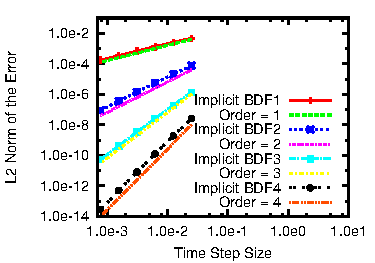
\includegraphics[scale=1.5]{figures/ImplicitBDF4}\caption{Order of accuracy for the SinCos Problem (Section~\ref{rythmos:sec:SinCos-Problem})
using Implicit BDF.}
\end{figure}

